\documentclass[12pt, a4paper]{article}

\usepackage[a4paper, margin=2cm]{geometry}
\usepackage{setspace}
\usepackage[portuguese]{babel}
\usepackage{graphicx}
\usepackage{hyperref}
\usepackage{amsfonts}
\usepackage[dvipsnames]{xcolor}

\chardef\_=`_

\title{\textbf{LI3 - Relatório da Fase II - Grupo 12}}
\author{
    Humberto Gomes (A104348) \\
    José Lopes     (A104541) \\
    José Matos     (A100612) \\
}
\date{janeiro de 2024}

\begin{document}
\maketitle
\onehalfspacing
\setlength{\parskip}{\baselineskip}
\setlength{\parindent}{0pt}

\begin{abstract}
    Após a conclusão da primeira fase deste trabalho, procurámos implementar as funcionalidades em
    falta para a conclusão do desenvolvimento desta aplicação: as restantes quatro
    \emph{queries}, um modo de uso interativo (uma interface TUI), testes funcionais e de
    desempenho, e suporte para um \emph{dataset} de maior dimensão, mantendo um desempenho
    aceitável. Adicionalmente, procurámos também melhorar o encapsulamento e a modularidade no
    nosso projeto.
\end{abstract}

\section{Estrutura do trabalho}

Nesta secção, procuramos descrever as diferenças entre a nossa arquitetura modular atual, e a que
tínhamos presente na primeira fase do projeto. Devido ao elevado número de módulos, após o diagrama
de dependências completo que se segue, este documento descreve o funcionamento de cada subsistema
lógico do programa um a um. Nestes esquemas, para reduzir a complexidade visual, não incluímos
todas as relações de dependência, mas apenas as mais relevantes. Segue-se a nossa convenção gráfica:

\begin{itemize}
    \item Um retângulo com cantos arredondados representa uma estrutura de dados;
    \item Um retângulo sem cantos arredondados representa um módulo cuja tarefa principal é a
          execução de código. No entanto, alguns destes módulos podem conter estruturas de dados
          auxiliares (por exemplo, uma gramática definida no módulo de um \emph{parser});
    \item $A \rightarrow B$ significa que o módulo $A$ depende do módulo $B$.
          % $A \dashrightarrow B$ representa uma falsa dependência, por exemplo, a necessidade de se
          % saber da existência de um nome de um tipo opaco.
    \item Qualquer módulo ou relação de dependência representado(a) a {\color{ForestGreen}verde}
          indica que o(a) mesmo(a) é uma adição nesta segunda fase, ausente na entrega anterior.
\end{itemize}

% TODO - inserir diagrama global aqui

\subsection{\emph{Parsing}}
\label{sec:parsing}

\begin{figure}[ht]
    \centering
    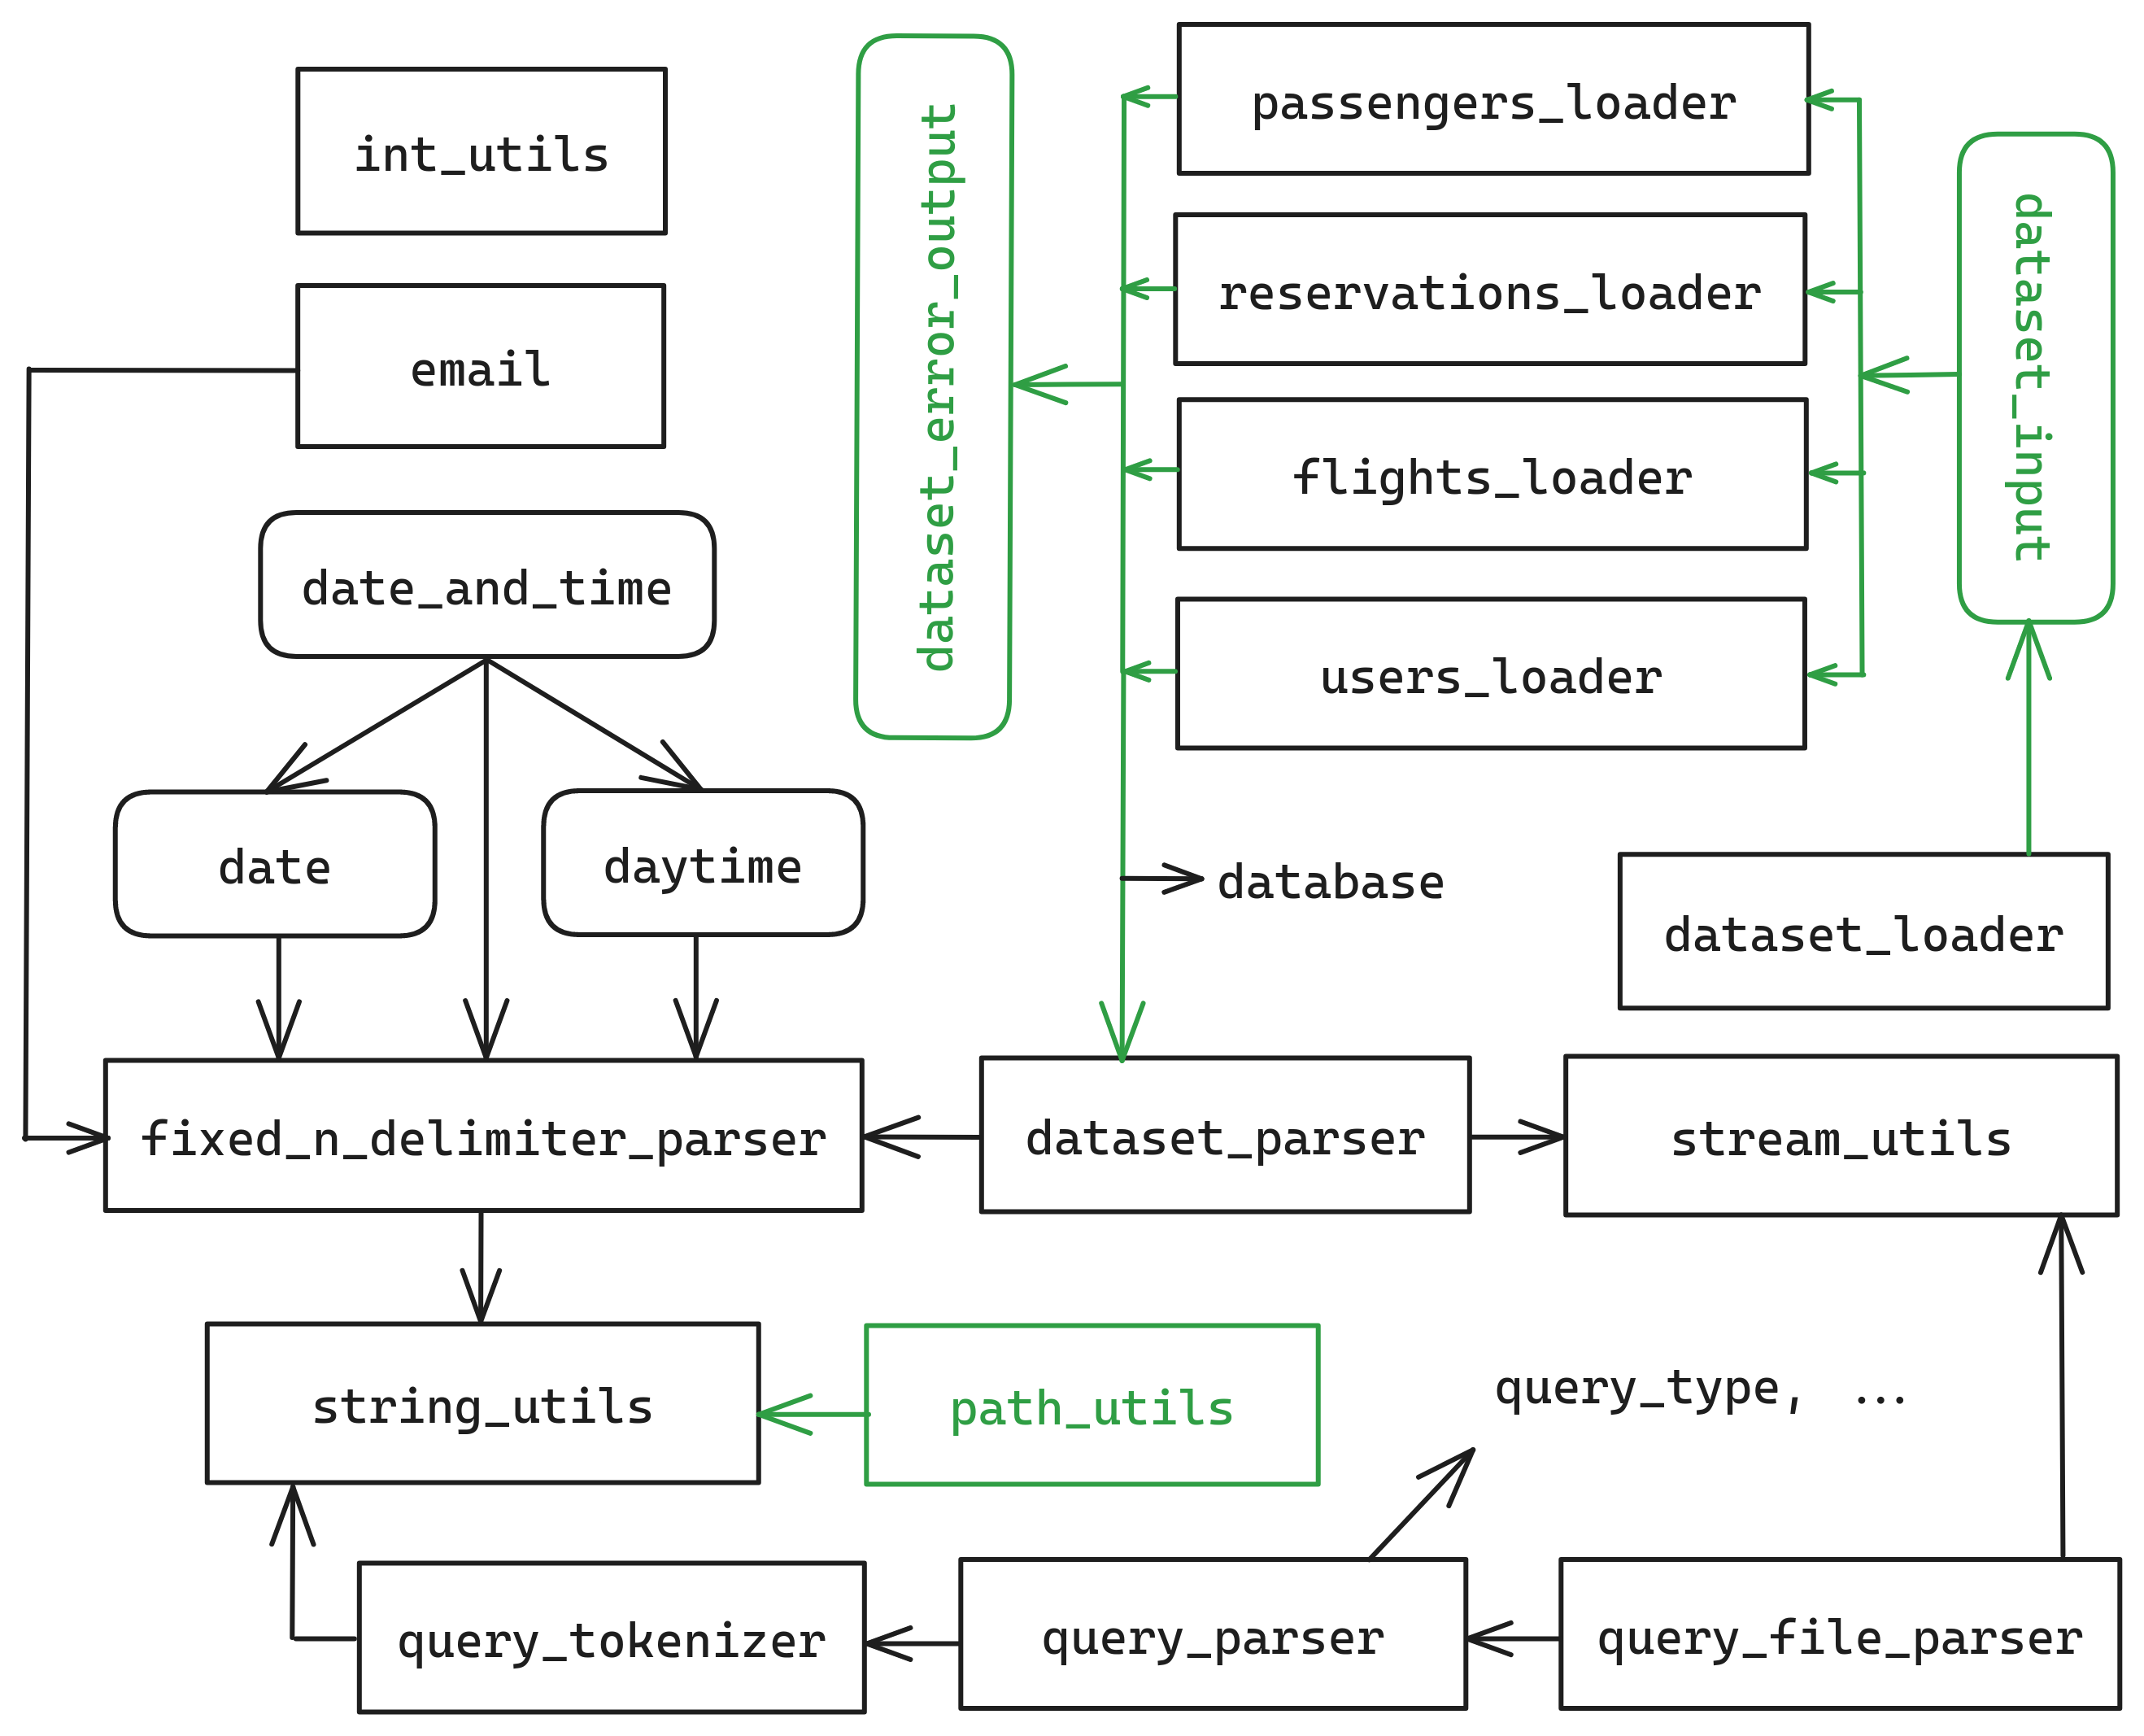
\includegraphics[scale=0.17]{res-fase2/parsing.png}
    \caption{Diagrama de dependências do subsistema de \emph{parsing}}
    \label{fig:parsing}
\end{figure}

Nesta fase do projeto, separámos as funcionalidades de \emph{input} de dados e \emph{output} de
erros num \emph{dataset}, antes concentradas no módulo \texttt{dataset\_loader}. Agora, este módulo
gere duas estruturas de dados distintas, \texttt{dataset\_input} e \texttt{dataset\_error\_output},
formadas por \emph{handles} de ficheiros abertos para leitura / escrita. Ademais, adicionámos o
módulo \texttt{path\_utils}, para manipulação de caminhos para ficheiros.

\end{document}
